% Options for packages loaded elsewhere
\PassOptionsToPackage{unicode}{hyperref}
\PassOptionsToPackage{hyphens}{url}
\documentclass[
  english,
  man,floatsintext]{apa6}
\usepackage{xcolor}
\usepackage{amsmath,amssymb}
\setcounter{secnumdepth}{-\maxdimen} % remove section numbering
\usepackage{iftex}
\ifPDFTeX
  \usepackage[T1]{fontenc}
  \usepackage[utf8]{inputenc}
  \usepackage{textcomp} % provide euro and other symbols
\else % if luatex or xetex
  \usepackage{unicode-math} % this also loads fontspec
  \defaultfontfeatures{Scale=MatchLowercase}
  \defaultfontfeatures[\rmfamily]{Ligatures=TeX,Scale=1}
\fi
\usepackage{lmodern}
\ifPDFTeX\else
  % xetex/luatex font selection
\fi
% Use upquote if available, for straight quotes in verbatim environments
\IfFileExists{upquote.sty}{\usepackage{upquote}}{}
\IfFileExists{microtype.sty}{% use microtype if available
  \usepackage[]{microtype}
  \UseMicrotypeSet[protrusion]{basicmath} % disable protrusion for tt fonts
}{}
\makeatletter
\@ifundefined{KOMAClassName}{% if non-KOMA class
  \IfFileExists{parskip.sty}{%
    \usepackage{parskip}
  }{% else
    \setlength{\parindent}{0pt}
    \setlength{\parskip}{6pt plus 2pt minus 1pt}}
}{% if KOMA class
  \KOMAoptions{parskip=half}}
\makeatother
% Make \paragraph and \subparagraph free-standing
\makeatletter
\ifx\paragraph\undefined\else
  \let\oldparagraph\paragraph
  \renewcommand{\paragraph}{
    \@ifstar
      \xxxParagraphStar
      \xxxParagraphNoStar
  }
  \newcommand{\xxxParagraphStar}[1]{\oldparagraph*{#1}\mbox{}}
  \newcommand{\xxxParagraphNoStar}[1]{\oldparagraph{#1}\mbox{}}
\fi
\ifx\subparagraph\undefined\else
  \let\oldsubparagraph\subparagraph
  \renewcommand{\subparagraph}{
    \@ifstar
      \xxxSubParagraphStar
      \xxxSubParagraphNoStar
  }
  \newcommand{\xxxSubParagraphStar}[1]{\oldsubparagraph*{#1}\mbox{}}
  \newcommand{\xxxSubParagraphNoStar}[1]{\oldsubparagraph{#1}\mbox{}}
\fi
\makeatother
\usepackage{graphicx}
\makeatletter
\newsavebox\pandoc@box
\newcommand*\pandocbounded[1]{% scales image to fit in text height/width
  \sbox\pandoc@box{#1}%
  \Gscale@div\@tempa{\textheight}{\dimexpr\ht\pandoc@box+\dp\pandoc@box\relax}%
  \Gscale@div\@tempb{\linewidth}{\wd\pandoc@box}%
  \ifdim\@tempb\p@<\@tempa\p@\let\@tempa\@tempb\fi% select the smaller of both
  \ifdim\@tempa\p@<\p@\scalebox{\@tempa}{\usebox\pandoc@box}%
  \else\usebox{\pandoc@box}%
  \fi%
}
% Set default figure placement to htbp
\def\fps@figure{htbp}
\makeatother
% definitions for citeproc citations
\NewDocumentCommand\citeproctext{}{}
\NewDocumentCommand\citeproc{mm}{%
  \begingroup\def\citeproctext{#2}\cite{#1}\endgroup}
\makeatletter
 % allow citations to break across lines
 \let\@cite@ofmt\@firstofone
 % avoid brackets around text for \cite:
 \def\@biblabel#1{}
 \def\@cite#1#2{{#1\if@tempswa , #2\fi}}
\makeatother
\newlength{\cslhangindent}
\setlength{\cslhangindent}{1.5em}
\newlength{\csllabelwidth}
\setlength{\csllabelwidth}{3em}
\newenvironment{CSLReferences}[2] % #1 hanging-indent, #2 entry-spacing
 {\begin{list}{}{%
  \setlength{\itemindent}{0pt}
  \setlength{\leftmargin}{0pt}
  \setlength{\parsep}{0pt}
  % turn on hanging indent if param 1 is 1
  \ifodd #1
   \setlength{\leftmargin}{\cslhangindent}
   \setlength{\itemindent}{-1\cslhangindent}
  \fi
  % set entry spacing
  \setlength{\itemsep}{#2\baselineskip}}}
 {\end{list}}
\usepackage{calc}
\newcommand{\CSLBlock}[1]{\hfill\break\parbox[t]{\linewidth}{\strut\ignorespaces#1\strut}}
\newcommand{\CSLLeftMargin}[1]{\parbox[t]{\csllabelwidth}{\strut#1\strut}}
\newcommand{\CSLRightInline}[1]{\parbox[t]{\linewidth - \csllabelwidth}{\strut#1\strut}}
\newcommand{\CSLIndent}[1]{\hspace{\cslhangindent}#1}
\ifLuaTeX
\usepackage[bidi=basic]{babel}
\else
\usepackage[bidi=default]{babel}
\fi
% get rid of language-specific shorthands (see #6817):
\let\LanguageShortHands\languageshorthands
\def\languageshorthands#1{}
\ifLuaTeX
  \usepackage[english]{selnolig} % disable illegal ligatures
\fi
\setlength{\emergencystretch}{3em} % prevent overfull lines
\providecommand{\tightlist}{%
  \setlength{\itemsep}{0pt}\setlength{\parskip}{0pt}}
% Manuscript styling
\usepackage{upgreek}
\captionsetup{font=singlespacing,justification=justified}

% Table formatting
\usepackage{longtable}
\usepackage{lscape}
% \usepackage[counterclockwise]{rotating}   % Landscape page setup for large tables
\usepackage{multirow}		% Table styling
\usepackage{tabularx}		% Control Column width
\usepackage[flushleft]{threeparttable}	% Allows for three part tables with a specified notes section
\usepackage{threeparttablex}            % Lets threeparttable work with longtable

% Create new environments so endfloat can handle them
% \newenvironment{ltable}
%   {\begin{landscape}\centering\begin{threeparttable}}
%   {\end{threeparttable}\end{landscape}}
\newenvironment{lltable}{\begin{landscape}\centering\begin{ThreePartTable}}{\end{ThreePartTable}\end{landscape}}

% Enables adjusting longtable caption width to table width
% Solution found at http://golatex.de/longtable-mit-caption-so-breit-wie-die-tabelle-t15767.html
\makeatletter
\newcommand\LastLTentrywidth{1em}
\newlength\longtablewidth
\setlength{\longtablewidth}{1in}
\newcommand{\getlongtablewidth}{\begingroup \ifcsname LT@\roman{LT@tables}\endcsname \global\longtablewidth=0pt \renewcommand{\LT@entry}[2]{\global\advance\longtablewidth by ##2\relax\gdef\LastLTentrywidth{##2}}\@nameuse{LT@\roman{LT@tables}} \fi \endgroup}

% \setlength{\parindent}{0.5in}
% \setlength{\parskip}{0pt plus 0pt minus 0pt}

% Overwrite redefinition of paragraph and subparagraph by the default LaTeX template
% See https://github.com/crsh/papaja/issues/292
\makeatletter
\renewcommand{\paragraph}{\@startsection{paragraph}{4}{\parindent}%
  {0\baselineskip \@plus 0.2ex \@minus 0.2ex}%
  {-1em}%
  {\normalfont\normalsize\bfseries\itshape\typesectitle}}

\renewcommand{\subparagraph}[1]{\@startsection{subparagraph}{5}{1em}%
  {0\baselineskip \@plus 0.2ex \@minus 0.2ex}%
  {-\z@\relax}%
  {\normalfont\normalsize\itshape\hspace{\parindent}{#1}\textit{\addperi}}{\relax}}
\makeatother

\makeatletter
\usepackage{etoolbox}
\patchcmd{\maketitle}
  {\section{\normalfont\normalsize\abstractname}}
  {\section*{\normalfont\normalsize\abstractname}}
  {}{\typeout{Failed to patch abstract.}}
\patchcmd{\maketitle}
  {\section{\protect\normalfont{\@title}}}
  {\section*{\protect\normalfont{\@title}}}
  {}{\typeout{Failed to patch title.}}
\makeatother

\usepackage{xpatch}
\makeatletter
\xapptocmd\appendix
  {\xapptocmd\section
    {\addcontentsline{toc}{section}{\appendixname\ifoneappendix\else~\theappendix\fi: #1}}
    {}{\InnerPatchFailed}%
  }
{}{\PatchFailed}
\makeatother
\keywords{Cognitive Control, Multi-Level Analysis, Decision-making, Cognition, Task-Switching, Stability-Flexibility, Experimental Effects, Within-Subject Dynamics, Individual Differences}
\usepackage{lineno}

\linenumbers
\usepackage{csquotes}
\usepackage{bookmark}
\IfFileExists{xurl.sty}{\usepackage{xurl}}{} % add URL line breaks if available
\urlstyle{same}
\hypersetup{
  pdftitle={Multi-level Analysis Of The Stability-Flexibility Dilemma},
  pdfauthor={Ulrich Mayr1, Sophia Vi Angleton1, Neha Nagarkar1, \& Dominik Graetz1},
  pdflang={en-EN},
  pdfkeywords={Cognitive Control, Multi-Level Analysis, Decision-making, Cognition, Task-Switching, Stability-Flexibility, Experimental Effects, Within-Subject Dynamics, Individual Differences},
  hidelinks,
  pdfcreator={LaTeX via pandoc}}

\title{Multi-level Analysis Of The Stability-Flexibility Dilemma}
\author{Ulrich Mayr\textsuperscript{1}, Sophia Vi Angleton\textsuperscript{1}, Neha Nagarkar\textsuperscript{1}, \& Dominik Graetz\textsuperscript{1}}
\date{}


\shorttitle{Multi-level Analysis Of The Stability-Flexibility Dilemma}

\authornote{

Add complete departmental affiliations for each author here. Each new line herein must be indented, like this line. NOTE put somewhere here that this study is part of a larger investigation funded by a grant from NIH

Enter author note here.

The authors made the following contributions. Ulrich Mayr: Conceptualization, Writing - Review \& Editing, Project Administration, Supervision; Sophia Vi Angleton: Writing - Original Draft Preparation, Writing - Review \& Editing, Formal Analysis, Visualization; Neha Nagarkar: Writing - Review \& Editing, Formal Analysis, Visualization; Dominik Graetz: Writing - Review \& Editing, Formal Analysis, Visualization.

Correspondence concerning this article should be addressed to Ulrich Mayr, Lewis Integrative Science Building, room 350 Eugene, OR 97403-1227. E-mail: \href{mailto:mayr@uoregon.edu}{\nolinkurl{mayr@uoregon.edu}}

}

\affiliation{\vspace{0.5cm}\textsuperscript{1} University of Oregon}

\abstract{%
A dominant view in cognitive control research concerning stability and flexibility is that of a tradeoff relationship, where the more cognitively stable a task representation becomes the harder it is to flexibly switch to another task. Although widely replicated, this tradeoff account is typically supported using a single level of analysis of the experimental effects of switch cost as a degree of conflict blockwise (Egner, 2007; Goschke, 2000b, 2000a; Rogers \& Monsell, 1995). A smaller body of research supports a different account of stability-flexibility, where on the level of within-subject dynamics stability and flexibility are found to co-occur (Mayr, Kuhns, \& Hubbard, 2014). This raises the question that the stability--flexibility tradeoff seen through experimental level effects is not a fundamental property of cognitive control but may instead reflect the analytic level at which it is measured. Moreover, individual differences work hints at substantial variability in how people balance stability and flexibility, suggesting that the relationship may not be uniform across all individuals (Mayr \& Grätz, 2024).

The present study investigates where differences in the stability-flexibility dilemma arise through a multi-level analytic approach. Additionally, we take a more direct and sensitive approach to understanding cognitive control mechanisms through looking at the degree of control required pre- and post- task-switching. Across two experiments, we examined stability--flexibility dynamics at three analytic levels: experimental effects, within‑subject dynamics, and individual differences. We find that it indeed matters to what level stability-flexibility mechanisms are analyzed. Evidence for the co-occurrence of tradeoff and antitradeoff relationships are found on different levels of analysis, underscoring the importance of a multi-level approach when interpreting stability-flexibility interactions. By showing that stability--flexibility dynamics vary across analytic scales, our results challenge the presumed ubiquity of the dominant tradeoff view and highlight the necessity of multi‑level approaches for understanding the mechanisms that govern cognitive control.
}



\begin{document}
\maketitle

\section{Introduction}\label{introduction}

A dominant view in research on cognitive control holds that adjustments of control are constrained by a general stability-flexibility tradeoff. Specifically, increasing the stability of a task-relevant representation makes flexible changes of that representation more difficult (Goschke, 2000b). You may be planning to give a speech for example, relying on your notes helps you stay on message reflecting high stability, but it can also make it harder to smoothly switch into an improvised, conversational mode when a question arises thereby reducing flexibility. The very thing that keeps you anchored can also slow you down when you need to pivot. Understanding stability-flexibility mechanisms is also of vital importance in the clinical world, with impaired regulation of cognitive control being implicated in various neurodevelopmental disorders such as attention deficit hyperactivity disorder, cerebral palsy, and autism spectrum disorder (Cepeda, Cepeda, \& Kramer, 2000; D'Cruz et al., 2013; Tajik‐Parvinchi, Farmus, Tablon Modica, Cribbie, \& Weiss, 2021). In these cases, disruptions in cognitive control can manifest as either overly rigid behavior or excessive distractibility, underscoring the importance of understanding the mechanisms that support both maintaining and updating task-relevant representations.

Despite this importance, most empirical work has examined stability--flexibility dynamics using blockwise manipulations, contrasting ``stable'' versus ``flexible'' blocks, and has evaluated the tradeoff primarily at the experimental‑effects level, averaging across trials and participants (Egner, 2007; Goschke, 2000a; Rogers \& Monsell, 1995). This approach has been instrumental in establishing the classic tradeoff pattern, but it also limits what can be observed. Blockwise designs cannot capture moment‑to‑moment adjustments that occur as people move from one trial to the next, nor can they reveal whether stability and flexibility might co‑occur within individuals under certain conditions. As a result, the field may be missing critical dynamics that unfold at finer temporal scales.

To address this limitation, we take a more sensitive approach to capture switch-cost as a function of trial-by-trial shifts in control. Manipulating previous‑trial switch and post‑switch demands independently provides a more detailed and responsive measure of how stability and flexibility interact as opposed to only understanding stability-flexibility shifts in a blockwise manner. Across two experiments, we use a task-switching `shape' or `color' task with the inclusion of univalent (neutral) and bivalent (ambiguous) stimuli in order to understand stability-flexibility as a function of congruence. We examine these dynamics across three complementary levels of analysis: (1) experimental level, (2) within‑subject dynamics, and (3) individual differences. This multi‑level framework allows us to test whether the stability--flexibility tradeoff emerges consistently across analytic scales or whether different levels reveal different patterns. We begin first by introducing the analytic level with the widest body of prior research: experimental effects.

\subsection{Stability-Flexibility Tradeoff and Experimental Effects.}\label{stability-flexibility-tradeoff-and-experimental-effects.}

The prediction of a tradeoff relationship arises from connectionist models of cognitive control. The behavior of these models can be described within an ``attractor landscape'' \emph{(Fig. 1)} (Brown, Reynolds, \& Braver, 2007; Geddert \& Egner, 2022). In this framework, different task representations form basins in a state space, and the depth of a basin reflects how strongly a task is currently activated. A deeper basin corresponds to a more stable task state, but it also requires more ``energy'' to move out of, making task switching more difficult. One data pattern that is consistent with this tradeoff prediction arises when examining task-switch costs as a function of previous-trial conflict. High conflict on the previous trial is assumed to strengthen the currently active task representation, effectively deepening its basin. This increased stability should then make switching on the next trial harder, producing larger switch costs. Although much of the dominant narrative in cognitive control has been built around this tradeoff pattern (Goschke, 2000b), this pattern is surprisingly inconsistent when examining cognitive control at different levels of analysis outside of experimental effects (Brown et al., 2007; Geddert \& Egner, 2022; Mayr et al., 2014).

\begin{figure}

{\centering 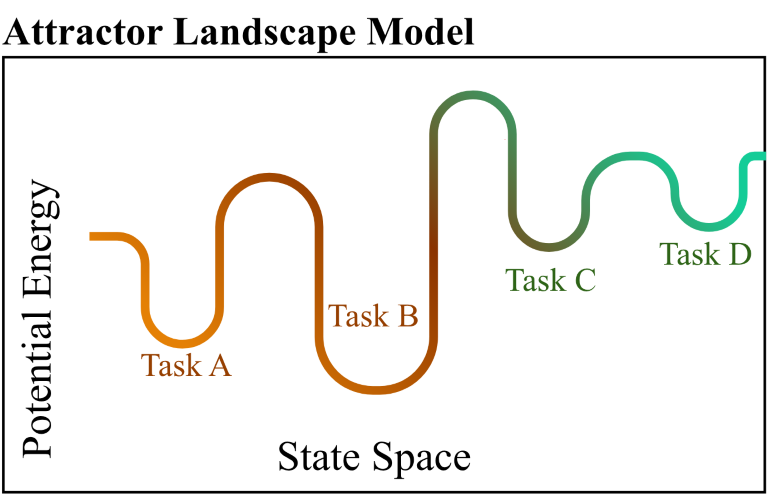
\includegraphics[width=0.5\linewidth]{sophia/predmodels} 

}

\caption{The landscape attractor model. This prediction model represents the dominant view of how stability-flexibility interact, which is in a tradeoff manner. Tasks are represented as basins of varying depth along a state space. The more stable a task representation is, the deeper the coorasponding basin in this attractor model. As a result for high stability, it takes more potential energy to move out of the task basin to a different task.}\label{fig:predmodels}
\end{figure}

\subsubsection{Experimental Level Hypotheses}\label{experimental-level-hypotheses}

Here we test whether experimental manipulations of previous and current trial control demands interact with the switch contrast in a manner that is consistent with a flexibility/stability tradeoff model.

\textbf{No-switch Trials.}

H1: Univalent trials (trials where one task is neutral) by definition have no conflict. Therefore, Univalent (Unambiguous) trials result in relatively shorter response times, and fewer errors compared to ambiguous.

H2: Bivalence (ambiguity) enforces stability because it introduces conflict resulting in longer reaction times and errors.

\textbf{Switch Trials.}

H1: Previous trial-group bivalence (ambiguity) enforces stability and should therefore cause higher switch costs (longer response times, more errors). If the previous group of trials was univalent (unambiguous), previous performance required less stability and should therefore reduce switch costs (lower response times, fewer errors).

H2: Current-trial bivalence requires establishing a stronger task set and therefore further increases RT and errors. Previous and current ambiguity should produce particularly large switch costs (e.g., an interaction between previous and current ambiguity).

\subsection{Stability-Flexibility Anti-Tradeoff Arises When Examining Within-Subject Dynamics.}\label{stability-flexibility-anti-tradeoff-arises-when-examining-within-subject-dynamics.}

note: this needs to be built on when interpreting the data more, read the mayr paper that finds co-occurance when analyzing within-sub dynamics in the meantime. Here we test whether trial-by-trial RT auto-correlations in combination with considering the experimental effects express a flexibility/stability tradeoff.

A recent reevaluation of the generalizability of the stability-flexibility tradeoff has posited that this negative tradeoff relationship may occur only in highly specified contexts (Mayr \& Grätz, 2024).These authors pointed toward a possible anti-tradeoff pattern, implying that cognitive stability and flexibility are both driven by a common factor and therefore can co-occur (Mayr et al., 2014). This paper adopts a more nuanced approach by examining when stability--flexibility dynamics emerge, weaken, or disappear. Across two experiments we conduct analysis on the experimental effects, within-subject dynamics, and individual differences level to identify the conditions under which tradeoffs arise and when they do not.

\begin{itemize}
\tightlist
\item
  note:\textbf{\emph{Cognitive Map Prediction Model.}} Contrary to predictions from the attractor model, there are recent hints suggesting the possibility of an anti-tradeoff pattern, where flexibility and stability appear to co-occur (Mayr et al., 2014; Morales, Moss, \& Mayr, 2022).
  In response to these results, Mayr and Graetz have suggested replacing the attractor-landscape perspective with a cognitive map conceptualization (Fig. 1B). Here, different tasks are locations within a task space that can be represented with varying degrees of resolution. The higher the resolution, the more stable tasks are encoded, but also the easier they are to find when switching, resulting in an anti-tradeoff pattern (Mayr \& Grätz, 2024).
  Despite some evidence for such anti-tradeoff patterns (Morales et al., 2022), this prediction has not been rigorously tested.
\end{itemize}

\subsection{Individual Differences.}\label{individual-differences.}

Here we test whether individual differences in measures of ``stability/efficiency'' and in measures of flexibility are consistent with the tradeoff model.
- tobias egner: individucal dif but looks at data in a block-wise manner.
found no relationship - study done in lab reference

note: we find an antitradeoff occuring, need to interpret the results for this section more too.
talk about age as a factor or not necessary for this paper?
maybe that can come in the discussion portion about other individual dif factors that we can explore with this level of analysis.

\subsubsection{Individual Differences Level Hypotheses}\label{individual-differences-level-hypotheses}

H1: We test the hypothesis derived from the tradeoff model that participants who are stable under a no-switch condition, which should be more challenging if the previous trials and/or the current trial is bivalent, should be less efficient on switch trials.

Because efficiency in almost all cognitive tasks is positively related (i.e., the ``positive manifold'') we will conduct a series of model tests, where on each level we will control for relationships occurring on ``preceding'' conditions to present less of a challenge to the stability-flexibility tradeoff.

H2: We predict that with an increase in stability demands (e.g., non-switch trials where the previous and/or current trial group were bivalent), the coefficients should turn negative in case of a tradeoff.

\section{Method}\label{method}

We report how we determined our sample size, all data exclusions (if any), all manipulations, and all measures in the study.

\subsection{Participants}\label{participants}

Our sample size for experiment 1 was 78, collected using convenience sampling methods. Our sample size for experiment 2 was 100, collected using convenience sampling methods. Both experiments pulled participants from the human subjects pool from the University of Oregon.

\subsection{Procedure}\label{procedure}

Participants signed an informed consent form given by our lab, then were instructed through the experiment ahead. Upon learning the instructions, participants completed one practice block, then proceeded to the start of the experiment. Upon completion of the experiment, subjects were debriefed and thanked for their time.

\subsubsection{Experiment 1}\label{experiment-1}

\textbf{Tasks and Stimuli.} There were 3 possible colors (red, green, blue) and 3 possible shapes (circle, square, and triangle). Additionally, there was a univalent color (gray) and a univalent shape (cross), which made up the fourth stimulus. The univalent stimuli always occurred within the groups of 3 trials. In no condition was a grey cross shown. In each group, the task remained to be univalent or bivalent, with a task switch after each group. Therefore, for each group of 3 trials, the currently irrelevant task could be either univalent or bivalent, and remained the same per group.

\textbf{Design.} The experiment was a task switching paradigm, wherein participants switched between a color and a shape task. In each trial, participants performed one of two tasks- color or shape, where they identify the color or shape of the stimulus, respectively. The task switches every three trials. In other words, the color or shape tasks were active for three consecutive trials. Three trials make up a group. Thus, the first trial of a group marks a task switch into the other task, the following two trials are task repetitions. There was a 100 ms Inter-trial-interval. The participants performed one initial practice block with 126 trials and then moved onto performing 5 experimental blocks with 120 trials each.

\subsubsection{Experiment 2}\label{experiment-2}

\textbf{Tasks and Stimuli.} The task involved the subject viewing a colored shape. There were 3 possible colors (red, green, blue) and 3 possible shapes (circle, square, and triangle). Additionally, there was a univalent color (gray) and a univalent shape (cross), which made up the fourth stimulus. In no condition both univalent dimensions were shown. Per trial, subjects completed one of two tasks, one task, ``color'' determined what color the stimuli is and ``shape'', determined the shape of the presented stimuli.

\textbf{Design.} Similar to experiment 1, subjects performed one of two tasks indicated by task instructions ``color'' or ``shape'', where they identified either the color or shape attribute of a presented stimulus. The task switched every 4 trials, where the first trial of every group always marked a task switch into another group of 4 trials. Similar to the alternate cues experimental design, the univalent aspect was manipulated randomly in a between trial groups design, in this case with all four trials in one group being bivalent or all four trials in one group being univalent, so that the participants knew that the stimuli alternated task dimension in groups of four. Subjects completed a total of 8 blocks excluding a practice block, each block containing 112 trials.

\subsection{Measures}\label{measures}

first introduce the measure then describe below
outcome measure first (iv)
predictor measure second

\subsection{Analysis Plan}\label{analysis-plan}

We used R (Version 4.5.2; R Core Team, 2025) and the R-packages \emph{dplyr} (Version 1.1.4; \textbf{R-dplyr?}), \emph{forcats} (Version 1.0.1; \textbf{R-forcats?}), \emph{ggplot2} (Version 4.0.1; \textbf{R-ggplot2?}), \emph{hausekeep} (Version 0.0.0.9003; \textbf{R-hausekeep?}), \emph{hlmer} (Version 0.1.0; \textbf{R-hlmer?}), \emph{janitor} (Version 2.2.1; \textbf{R-janitor?}), \emph{lme4} (Version 1.1.38; \textbf{R-lme4?}), \emph{lmerTest} (Version 3.2.0; \textbf{R-lmerTest?}), \emph{lubridate} (Version 1.9.4; \textbf{R-lubridate?}), \emph{Matrix} (Version 1.7.4; \textbf{R-Matrix?}), \emph{papaja} (Version 0.1.4; Aust \& Barth, 2025), \emph{psych} (Version 2.5.6; \textbf{R-psych?}), \emph{purrr} (Version 1.2.0; \textbf{R-purrr?}), \emph{readr} (Version 2.1.6; \textbf{R-readr?}), \emph{rio} (Version 1.2.4; \textbf{R-rio?}), \emph{sjPlot} (Version 2.9.0; \textbf{R-sjPlot?}), \emph{stringr} (Version 1.6.0; \textbf{R-stringr?}), \emph{tibble} (Version 3.3.0; \textbf{R-tibble?}), \emph{tidyr} (Version 1.3.2; \textbf{R-tidyr?}), \emph{tidyverse} (Version 2.0.0; \textbf{R-tidyverse?}), and \emph{tinylabels} (Version 0.2.5; Barth, 2025) for all our analyses.
layout how we conducted our analyses

\section{Results}\label{results}

no interpretations here KISS

figures for experimental effects and for third level effects, prob no vis for within subject level

\section{Discussion}\label{discussion}

prelim findings: across both experiments, not a strong indication of a tradeoff pattern, not consistent between models across experiments but some models show antitradeoff relationships occuring. in mine, drift rate shows an antitradeoff (pos effect in v = antitradeoff). in within sub, we want to focus moreso on the added affects (more complex effects) becusae the predictors that are seen also in the experiemental model are not as interpretable here in the within sub model as the full predictor

drift rate on lm models are good results and consistent across RT and error

\newpage

\section{References}\label{references}

\phantomsection\label{refs}
\begin{CSLReferences}{1}{0}
\bibitem[\citeproctext]{ref-R-papaja}
Aust, F., \& Barth, M. (2025). \emph{{papaja}: {Prepare} reproducible {APA} journal articles with {R Markdown}}. \url{https://doi.org/10.32614/CRAN.package.papaja}

\bibitem[\citeproctext]{ref-R-tinylabels}
Barth, M. (2025). \emph{{tinylabels}: Lightweight variable labels}. \url{https://doi.org/10.32614/CRAN.package.tinylabels}

\bibitem[\citeproctext]{ref-brown_2007_a}
Brown, J. W., Reynolds, J. R., \& Braver, T. S. (2007). A computational model of fractionated conflict-control mechanisms in task-switching. \emph{Cognitive Psychology}, \emph{55}, 37--85. \url{https://doi.org/10.1016/j.cogpsych.2006.09.005}

\bibitem[\citeproctext]{ref-cepeda_2000_task}
Cepeda, N. J., Cepeda, M. L., \& Kramer, A. F. (2000). Task switching and attention deficit hyperactivity disorder. \emph{Journal of Abnormal Child Psychology}, \emph{28}, 213--226. \url{https://doi.org/10.1023/a:1005143419092}

\bibitem[\citeproctext]{ref-dcruz_2013_reduced}
D'Cruz, A.-M., Ragozzino, M. E., Mosconi, M. W., Shrestha, S., Cook, E. H., \& Sweeney, J. A. (2013). Reduced behavioral flexibility in autism spectrum disorders. \emph{Neuropsychology}, \emph{27}, 152--160. \url{https://doi.org/10.1037/a0031721}

\bibitem[\citeproctext]{ref-egner_2007_congruency}
Egner, T. (2007). Congruency sequence effects and cognitive control. \emph{Cognitive, Affective, \& Behavioral Neuroscience}, \emph{7}, 380--390. \url{https://doi.org/10.3758/cabn.7.4.380}

\bibitem[\citeproctext]{ref-geddert_2022_no}
Geddert, R., \& Egner, T. (2022). No need to choose: Independent regulation of cognitive stability and flexibility challenges the stability-flexibility trade-off. \emph{Journal of Experimental Psychology: General}. \url{https://doi.org/10.1037/xge0001241}

\bibitem[\citeproctext]{ref-goschke_2000_14}
Goschke, T. (2000a). \emph{14 intentional reconfiguration and involuntary persistence in task set switching}.

\bibitem[\citeproctext]{ref-goschke_2000_intentional}
Goschke, T. (2000b). Intentional reconfiguration and involuntary persistence in task-set switching. \emph{Attention and Performance}, \emph{18}. Retrieved from \url{https://www.researchgate.net/publication/38140172_Intentional_reconfiguration_and_involuntary_persistence_in_task-set_switching}

\bibitem[\citeproctext]{ref-mayr_2024_does}
Mayr, U., \& Grätz, D. (2024). Does cognitive control have a general stability/flexibility tradeoff problem? \emph{Current Opinion in Behavioral Sciences}, \emph{57}, 101389. \url{https://doi.org/10.1016/j.cobeha.2024.101389}

\bibitem[\citeproctext]{ref-mayr_2014_longterm}
Mayr, U., Kuhns, D., \& Hubbard, J. (2014). Long-term memory and the control of attentional control. \emph{Cognitive Psychology}, \emph{72}, 1--26. \url{https://doi.org/10.1016/j.cogpsych.2014.02.001}

\bibitem[\citeproctext]{ref-morales_2022_age}
Morales, P., Moss, M. E., \& Mayr, U. (2022). Age differences in the recovery from interruptions. \emph{Psychology and Aging}, \emph{37}, 816--826. \url{https://doi.org/10.1037/pag0000706}

\bibitem[\citeproctext]{ref-R-base}
R Core Team. (2025). \emph{R: A language and environment for statistical computing}. Vienna, Austria: R Foundation for Statistical Computing. Retrieved from \url{https://www.R-project.org/}

\bibitem[\citeproctext]{ref-rogers_1995_costs}
Rogers, R. D., \& Monsell, S. (1995). Costs of a predictible switch between simple cognitive tasks. \emph{Journal of Experimental Psychology: General}, \emph{124}, 207--231. \url{https://doi.org/10.1037/0096-3445.124.2.207}

\bibitem[\citeproctext]{ref-tajikparvinchi_2021_the}
Tajik‐Parvinchi, D., Farmus, L., Tablon Modica, P., Cribbie, R. A., \& Weiss, J. A. (2021). The role of cognitive control and emotion regulation in predicting mental health problems in children with neurodevelopmental disorders. \emph{Child: Care, Health and Development}, \emph{47}, 608--617. \url{https://doi.org/10.1111/cch.12868}

\end{CSLReferences}


\end{document}
